%%%%%%%%%%%%%%%%%%%%%%%%%
% Dokumentinformationen %
%%%%%%%%%%%%%%%%%%%%%%%%%
\newcommand{\titleinfo}{Wechsel- \& Drehstromtechnik - Formelsammlung}
\newcommand{\authorinfo}{Braun \& Co, J.Rast}
\newcommand{\versioninfo}{$Revision: 1 $ - powered by \LaTeX}

%%%%%%%%%%%%%%%%%%%%%%%%%%%%%%%%%%%%%%%%%%%%%
% Standard projektübergreifender Header für
% - Makros 
% - Farben
% - Mathematische Operatoren
%
% DORT NUR ERGÄNZEN, NICHTS LÖSCHEN
%%%%%%%%%%%%%%%%%%%%%%%%%%%%%%%%%%%%%%%%%%%%%
%Schriftgr"osse, Layout, Papierformat, Art des Dokumentes
\documentclass[10pt,a4paper,fleqn,headsepline,footsepline]{scrartcl}
%Einstellungen der Seitenränder
\usepackage[left=0.8cm,right=0.8cm,top=0.5cm,bottom=0.5cm,includeheadfoot]{geometry}
% Sprache, Zeichensatz, packages
\usepackage[UTF8]{inputenc}
\usepackage[ngerman]{babel,varioref}
\usepackage{amssymb,amsmath,graphicx,xcolor,lastpage,wrapfig,verbatim}
\usepackage{tabularx}
\usepackage{multicol}
\usepackage{rotating}
\usepackage{floatflt}
\usepackage{array}
\usepackage{scrlayer-scrpage}
\usepackage{multirow,multicol}
\usepackage{trfsigns, trsym}
\usepackage{tikz}
\usepackage{afterpage}


\usepackage[european]{circuitikz}
\usetikzlibrary{patterns}
\pgfdeclarelayer{bg}    % declare background layer
\pgfsetlayers{bg,main}
\newcommand*{\rechterWinkelRadius}{.25cm}
\newcommand*{\rechterWinkel}[2]{% #1 = point, #2 = start angle
   \draw[shift={(#2:\rechterWinkelRadius)}] (#1) arc[start angle=#2, delta angle=90, radius = \rechterWinkelRadius];
   \fill[shift={(#2+45:\rechterWinkelRadius/2)}] (#1) circle[radius=1.25\pgflinewidth];
}


\usepackage{adjustbox}
%
\setkomafont{pageheadfoot}{\footnotesize}
%
%
\RedeclareSectionCommands[
  beforeskip=-.2\baselineskip,
  afterskip=.1\baselineskip
]{section,subsection,subsubsection,paragraph}

\definecolor{pgrey}{rgb}{0.2,0.2,0.2}
\definecolor{black}{rgb}{0,0,0}
\definecolor{red}{rgb}{1,0,0}
\definecolor{white}{rgb}{1,1,1}
\definecolor{grey}{rgb}{0.8,0.8,0.8}
\definecolor{green}{rgb}{0,.8,0.05}
\definecolor{brown}{rgb}{0.603,0,0}

\DeclareMathOperator{\sinc}{sinc}
\DeclareMathOperator{\sgn}{sgn}
\DeclareMathOperator{\Real}{Re}
\DeclareMathOperator{\Imag}{Im}
%\DeclareMathOperator{\e}{e}
\DeclareMathOperator{\cov}{cov}
\DeclareMathOperator{\PolyGrad}{PolyGrad}


\newcommand{\HRule}{\noindent\rule{\linewidth}{1pt}}


\newcommand{\matlab}[1]{\footnotesize{(Matlab: \texttt{#1})}\normalsize{}}
\newcommand{\skript}[1]{${\textcolor{pgrey}{\mbox{\small{Skript S.#1}}}}$}
\newcommand{\kuchling}[1]{$_{\textcolor{red}{\mbox{\small{Kuchling #1}}}}$}
\newcommand{\stoecker}[1]{$_{\textcolor{orange}{\mbox{\small{Stöcker #1}}}}$}
\newcommand{\sachs}[1]{$_{\textcolor{blue}{\mbox{\small{Sachs S. #1}}}}$}
\newcommand{\hartl}[1]{$_{\textcolor{green}{\mbox{\small{Hartl S. #1}}}}$}

%
\newcommand{\myparagraph}[1]{\paragraph{#1}\mbox{}\\\nopagebreak}
\newcommand{\formelbuch}[1]{$\quad{\textcolor{pgrey}{\mbox{\small{S#1}}}}$}

\newcommand*{\diff}{\mathop{}\!\mathrm{d}}

\newcommand{\arraystretchOriginal}{1.5}

\newcommand{\FT}
{
\begin{picture}(1,0.5)
\put(0.2,0.1){\circle{0.14}}\put(0.27,0.1){\line(1,0){0.5}}\put(0.77,0.1){\circle*{0.14}}
\end{picture}
}

\renewcommand{\arraystretch}{\arraystretchOriginal}


\newcolumntype{L}[1]{>{\raggedright\let\newline\\\arraybackslash\hspace{0pt}}m{#1}}
\newcolumntype{C}[1]{>{\centering\let\newline\\\arraybackslash\hspace{0pt}}m{#1}}
\newcolumntype{R}[1]{>{\raggedleft\let\newline\\\arraybackslash\hspace{0pt}}m{#1}}


\author{\authorinfo}
\title{\titleinfo}
%
%Kopf- und Fusszeile
%
\lohead*{\titleinfo}
\rohead*{\today}
\lofoot*{\authorinfo}
\cofoot*{}
\rofoot*{Seite \thepage { }von \pageref{LastPage}}
%
\pagestyle{scrheadings}



% TikZ zeugs:
\usepackage{circuitikz}
\usetikzlibrary{patterns}
\pgfdeclarelayer{bg}    % declare background layer
\pgfsetlayers{bg,main}
\newcommand*{\rechterWinkelRadius}{.25cm}
\newcommand*{\rechterWinkel}[2]{% #1 = point, #2 = start angle
   \draw[shift={(#2:\rechterWinkelRadius)}] (#1) arc[start angle=#2, delta angle=90, radius = \rechterWinkelRadius];
   \fill[shift={(#2+45:\rechterWinkelRadius/2)}] (#1) circle[radius=1.25\pgflinewidth];
}


\usepackage{adjustbox}

% M\"oglichst keine Erg\"anzungen hier, sondern in header.tex
\begin{document}

%%%%%%%%%%%%%%%%%%%%%%%%%%%%%%%%%%%%%%%%%%%%%%%%%%%%%%%%%%%%%%%%%%%%%%%%%%%%%%%%%%%%%%%%%%%%%%%%


\section{Wechselstromtechnik}
	\subsection{Periodisch zeitabh\"angige Gr\"ossen}
 %		\subsubsection{Periodische Schwingungen}
 %			\begin{tabular}{p{6cm}p{4.5cm}p{7.5cm}}
 %				Frequenz &
 %           		\fbox{$f = \frac{1}{T} = \frac{2 \pi}{\omega}$} &
 %            		$[f] = s^{-1}$ \\ \\
 %				Schwingungsbreite &
 %					\fbox{$i_{pp} = i_{max} - i_{min}$} \\ \\
 %				Scheitelwert &
 %					\fbox{$\hat{i} = |i_{max}| \quad\text{für}\quad{|i_{max}|}\geq{|i_{min}|} \quad \text{oder} \quad \hat{i} = |i_{min}|\quad\text{für}\quad |i_{max}| < |i_{min}|$}
 %			\end{tabular}
		

		\subsubsection{Mittelwerte periodischer Gr\"ossen}
			\begin{tabular}{|p{5.5cm}|p{6cm}|p{6.5cm}|}
			\hline
				Arithmetischer Mittelwert, Gleichwert, Linearer MW &
				$X_0 = \overline{X} = X_m = \frac {1} {T} \int\limits_{t_0}^{t_0+T} x(t)dt$ &
				Ist die Fl\"ache unter der Zeitfunktion \"uber eine Periode. \\
			\hline
				MW des Quadrates, Leistung &
				$X^2 = \frac {1} {T} \int\limits_{t_0}^{t_0+T} x^2(t)dt$ & 
				$X^n = \frac {1} {T} \int\limits_{t_0}^{t_0+T} x^n(t)dt$ (MW $n$. Ordnung) \\
			\hline
				Effektivwert, Quadratischer MW &
				$X = X_{\text{eff}}= \sqrt{X^2} = \sqrt{\frac{1}{T} \int\limits ^{t_0+T} _{t_0}{x^2(t)dt}}$
				& \\ 
			\hline
				Gleichrichtwert &
				$X_{|m|} = \bar{|X|} = \frac{1}{T} \int\limits_{t_0}^{t_0+T}{|x(t)| dt}$ &
				Arithm. Mittelwert der Zweiweggleichrichterschaltung \\
			\hline				    
				Energie der Periode $T$ &
				$W_T = \int\limits_{t_0}^{t_0+T}{P(t) dt}$ &
				ist die Energie positiv, nimmt der Zweipol Energie auf \\
			\hline                    
				Wirkleistung &
				$P = \frac{1}{T} \int\limits_{t_0}^{t_0+T}{P(t) dt}  = \frac{X^2}{R}$ & \\
			\hline
			\end{tabular}
			
	\subsubsection{Verhältnisszahlen}
		\begin{multicols}{2}
			\begin{tabular}{ll}
				Scheitelfaktor $k_s$ (crest factor): 
					& $k_s = \frac{\text{Scheitelwert}} 	
							{\text{Effektivwert}} = \frac{\hat{x}}{X}$ \\
   				Formfaktor F (form factor): 
   				 	& $F = \frac{\text{Effektivwert}}
   				 			{\text{Gleichrichtwert}} = \frac{X}{|\bar{x}|}$ \\	
   				Klirrfaktor k: 
   				    & $k = \frac{\text{Effektivwert der 	
   				    					Oberwellen}}
   				    		{\text{Gesamteffektivwert}}$ \\
			\end{tabular}
			\columnbreak
	
			\begin{tabular}{ll}
				Schwingungsgehalt: 
					& $s = \frac{\text{Effektivwert des 	
										Wechselanteils}}
							{\text{Effektivwert der 		
									Mischgr\"osse}}$ \\
				Effektive Welligkeit:
					 & $\frac{\text{Effektivwert des 		
					 				Wechselanteils}}
					 		{\text{Gleichwert der 	
					 				Mischgr\"osse}}$ \\
				Riffelfaktor: 
					& $\frac{\text{Scheitelwert des 	
									Wechselanteils}}
							{\text{Gleichwert der 
									Mischgr\"osse}}$ \\
			\end{tabular}
		\end{multicols}

		\begin{tabular}{p{6.5cm}p{3cm}p{7.5cm}}
			\textbf{Simpsonsche Regel}
				&	Gleichwert: &
						$\bar{x} = \frac{\Delta t}{3T} \sum m \cdot x$ \\ 
				\textit{(Berechnungsmethode anhand}		\\
				
				\textit{eines Graphen) }
				 &	Gleichrichtwert: &
						$|\bar{x}| = \frac{\Delta t}{3T} \sum m \cdot |x|$ \\ \\
						
				 &	Effektivwert: &
						$X_{eff} = \sqrt{\frac{\Delta t}{3T} \sum m \cdot x^2}$ \\ \\
				\begin{minipage}{10cm}
					\begin{tabular}{| c | c | c | c | c | c | c | c |}
						\hline
			 				$n$ & $t$ &$x$ & $x^2$ & $m$ & $m \cdot x$ & $m \cdot x^2$ \\
			 			\hline
				 			0 & & & & 1 & & \\
				 		\hline
				 			1 & & & & 4 & & \\
				 		\hline
				 			2 & & & & 2 & & \\
				 		\hline
				 			\vdots & & & & \vdots & & \\
				 		\hline
				 			n-1 & & & & 1 & & \\
				 		\hline
			 		\end{tabular}
				\end{minipage} &
				\begin{minipage}{12.5cm}
                	\begin{itemize}
                		\item Im Graph innerhald der Periode $T$ 	
                			  eine ungerade Anzahl von $\boldsymbol{n}$ \textbf{Stützstellen} in konstanten \textbf{Abst\"anden} $\boldsymbol{\Delta t}=\frac{T}{n-1}$ w\"ahlen. Mit $t = t_0$ und $t = t_0+T$ \\ 
                			  $\rightarrow$ Zur Kontrolle $x(t_0) = x(t_0+(n-1)\cdot\Delta t)$
                		\item An diesen Stützstellen jeweils den 
                			  Augenblickswert ablesen und in die Tabelle (siehe Links) eintragen.
                		\item Anschliessend die Tabelle vervollständigen und mit den obigen Formeln summieren
                		\item \textbf{Faktor} $\boldsymbol{m}$ 
                			  wird wie folgt gebildet: Für ungerade n ist m=4; bei der ersten und bei der
                			  letzten Stützstelle ist m=1, bei den übrigen ist m=2.    
                	\end{itemize}
                \end{minipage}
			\end{tabular}
	\subsubsection{Gleichrichterschaltungen}
			\begin{tabular}{p{4cm}p{4cm}p{9cm}}
            	\begin{minipage}{4cm}
            		\textbf{Einweggleichrichtung} \\
            		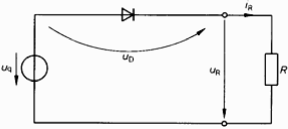
\includegraphics[height=1.2cm]{bilder/EinwegGleichrichtung.png}
            	\end{minipage} &
            		\begin{minipage}{4cm}
                    	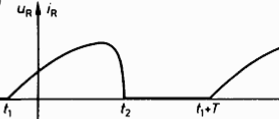
\includegraphics[width=4cm]{bilder/AusgangsspannungStromEinwegGleichrichtung.png}
                    \end{minipage} &
					\begin{minipage}{8cm}
                    	Fliesst nur ein Strom in Durchlassrichtung der Diode. \\
                    	Summe der Oberwellen $i_0=0.2176A$ \\
                    	$t_1 < t < t_2$ $\Rightarrow$ $u_R = u_q$ ; $i_R = u_q/R$ ; $u_D = 0$ \\
                    	$t_2 < t < (t_1+T)$ $\Rightarrow$ $u_R = 0$ ; $i_R = 0$ ; $u_D = u_q$
                    \end{minipage} \\
				\begin{minipage}{4cm}
                	\textbf{Zweiweggleichrichtung} \\
                	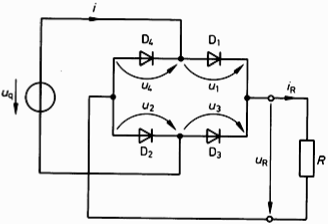
\includegraphics[height=1.5cm]{bilder/BrueckenGleichrichtung.png}
                \end{minipage} &
					\begin{minipage}{4cm}
                    	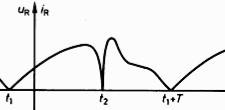
\includegraphics[width=4cm]{bilder/AusgangsspannungBrueckenGleichrichtung.png}
                    \end{minipage} &
					\begin{minipage}{9cm}
                    	Ausgangsspannung ist Betrag der Eingangsspannung. \\
                    	$t_1 < t < t_2$ $\Rightarrow$ $D_1,D_2$ leiten ; $D_3,D_4$ sperren \\
                    	$t_2 < t < (t_1+T)$ $\Rightarrow$ $D_1,D_2$ sperren ; $D_3,D_4$ leiten \\
                    	$u_R = |u_q|$ ; $i_R = u_R/R = |i|$
                    \end{minipage}
            \end{tabular}
	\subsection{Sinusf\"ormige Schwingungen von Spannung und Strom}
 		\subsubsection{Erzeugung sinusf\"ormiger Schwingungen}
 			\begin{minipage}{6cm}
 				\textbf{Lenzsche Regel}\\
 					Der induzierte Strom wirkt seiner Ursache entgegen.\\
 					Ursache des induzierten Stromes ist die \"Anderung des Flusses.
             \end{minipage}
             \hfill
 			\begin{minipage}{4.5cm}
 				\textbf{Bewegte Leiter im \\ homogenen Magnetfeld}\\
             	$U = B \cdot l \cdot v_q$ \\
             	             	$v_q = v \cdot cos\beta = v \cdot sin\alpha\\$
             	$U = \hat{U} \cdot sin \alpha$
             \end{minipage}
 			\begin{minipage}{3.5cm}
             	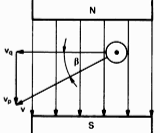
\includegraphics[width=3.5cm]{bilder/BewegteLeiter.png}
             \end{minipage}
 			\begin{minipage}{3.5cm}
             	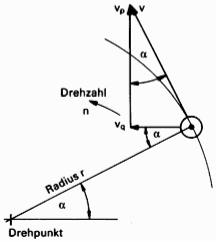
\includegraphics[width=3.5cm]{bilder/KreisfoermigeBewegung.png}
             \end{minipage}
% 		\subsubsection{Beschreibung sinusf\"ormiger Spannungen und Str\"ome}
% 			\begin{tabular}{p{6cm}p{4.5cm}p{7.5cm}}
%             	\textbf{Kreisfrequenz} &
%             		\fbox{$\omega = \frac{2 \pi}{T} = 2 \pi f$} &
%             		$[\omega] = s^{-1}$ \\ \\
%             	\textbf{Effektivwert für sinusf\"ormige Gr\"ossen} &
%             		\fbox{$U = \frac{\hat{u}}{\sqrt{2}} \quad I = \frac{\hat{i}}{\sqrt{2}}$}
%             \end{tabular}
		\subsubsection{Komplexe Zeiger}
			\begin{minipage}[t]{6cm}
            	\textbf{Prinzip der Zeigertechnik}
            \end{minipage}
			\begin{minipage}{6cm}
            	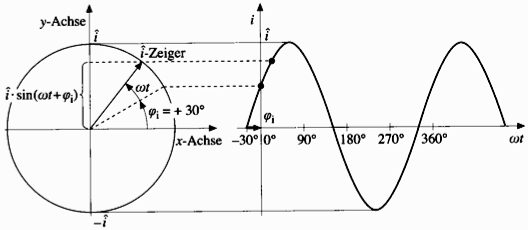
\includegraphics[width=6cm]{bilder/RotierenderScheitelwertzeiger.png}
            \end{minipage}
			\begin{minipage}{3.5cm}
            	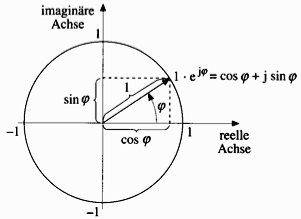
\includegraphics[width=3.5cm]{bilder/EulerscheRelation.png}
            \end{minipage} \\
			\begin{tabular}{p{4.0cm}p{5.5cm}p{8.5cm}}
            	Komplexer Effektivwert &
            		$\underline{U} = \frac{\underline{\hat{u}}}{\sqrt{2}}$ &
            		$\underline{U}$ = Kompl. Effektivwert, $\underline{\hat{u}}$ = Kompl. Scheitelwert \\
				Exponentialform &
					$\underline{\hat{u}} = \hat{u} \cdot e^{j\varphi_u} \quad \underline{U} = U \cdot e^{j\varphi_U}$  &
					$\varphi_U$ = Nullphasenwinkel der Spannung\\
				Algebraische Form &
					$\underline{\hat{u}} = \hat{u} (\cos(\varphi_u)+j\sin(\varphi_u))$ &
					$\Real(\underline{\hat{u}}) = \hat{u} \cdot \cos(\varphi_u)$ \quad $\Imag(\underline{\hat{u}}) = \hat{u} \cdot \sin(\varphi_u)$ \\
				&	$\underline{U} = U (\cos(\varphi_U)+j\sin(\varphi_U))$ &
					$\Real(\underline{U}) = U \cdot \cos(\varphi_U)$ \quad $\Imag(\underline{U}) = U \cdot \sin(\varphi_U)$ \\
				Umrechnung &
					$|\hat{u}| = \sqrt{\Real(\underline{\hat{u}})^2 + \Imag(\underline{\hat{u}})^2}$ \break $\varphi_u = \arctan\left(\dfrac{\Imag(\underline{\hat{u}})}{\Real(\underline{\hat{u}})}\right)$ \\
				&	$|U| = \sqrt{\Real(\underline{U})^2 + 		\Imag(\underline{U})^2}$ \break
					 $\varphi_u = \arctan\left(\dfrac{\Imag(\underline{U})}{\Real(\underline{U})}\right)$ \\
				Komplexe Drehzeiger & 	
					\multicolumn{2}{l}{$\underline{u}(t) = \underline{\hat{u}} \cdot e^{j\omega t} = \hat{u} \cdot e^{j\varphi_u} \cdot e^{j\omega t} = \hat{u} \cdot e^{j(\omega t + \varphi_u})$} \\
				Phasenwinkel & 
					$\varphi = \varphi_u - \varphi_i$ &
					$\varphi > 0$: $U$ eilt $I$ vor\\ 
				& 	$\varphi = \frac{\Delta t}{T}\cdot 2\pi$ &
					$\varphi < 0$: $U$ eilt $I$ nach\\
			\end{tabular}
		\subsubsection{Komponenten linearer Wechselstromnetzwerke}% \formelbuch{125}}
			\begin{tabular}{llll}
			$\underline{Z} = R +j X$: 
				& Komplexer Widerstand (Impedanz); 
				& $R$: Wirkwiderstand (Resistanz); 
				& $X$: Blindwiderstand (Reaktanz)\\
			$\underline{Y} = G + j B$: 
				& Komplexer Leitwert (Admittanz); 
				& $G$: Wirkleitwert (Konduktanz); 
				& $B$: Blindleitwert (Suszeptanz)
	      	\end{tabular} \\ \\
			\begin{tabular}{|l|l|l|l|l|l|ll|}
			\hline
				\textbf{Widerstand} & 
					\multicolumn{2}{l|}{$ \underline{Z}_R = R$} & \multicolumn{2}{l|}{$ \underline{Y}_R = G =\frac{1}{R}$} &
					&
					\parbox[c][0.8cm][c]{1cm}{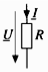
\includegraphics[height=1cm,angle=90]{bilder/Wirkwiderstand.png}}&
                	\parbox[c][0.8cm][c]{1cm}{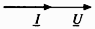
\includegraphics[width=1cm]{bilder/WirkwiderstandZeiger.png}} \\
			\hline	                    
				\textbf{Induktivit\"at} &
					$ \underline{Z}_L = j \omega L = j X_L$&
					$ X_L = \omega L$ &
					$ \underline{Y}_L = \frac{1}{j \omega L} = j B_L$ & 
					$ B_L = - \frac{1}{\omega L}$ &
					$ W_L=\frac12 L {I_L}^2$  &
					
		            \parbox[c][0.8cm][c]{1cm}{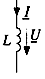
\includegraphics[height=1cm,angle=90]{bilder/Spule.png}}&
		            \parbox[c][1cm][c]{1cm}{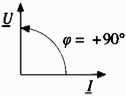
\includegraphics[width=1cm]{bilder/SpuleZeiger.png}}
		            \\
			\hline		                
				\textbf{Kondensator} &
					$ \underline{Z}_C = \frac{1}{j \omega C} = jX_C $ &
					$ X_C = - \frac{1}{\omega C} $ &
					$ \underline{Y}_C = j \omega C = j B_C $&
					$ B_C = \omega C $ &
					$ W_C=\frac12 C {U_C}^2$ & 
		            \parbox[c][0.8cm][c]{0.8cm}{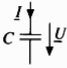
\includegraphics[height=0.9cm,angle=90]{bilder/Kondensator.png}}&
		            \parbox[c][1cm][c]{1cm}{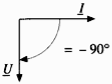
\includegraphics[width=1cm]{bilder/KondensatorZeiger.png}}\\
			\hline	    
				\parbox[c][1cm][c]{2cm}{}&
					\multicolumn{2}{l|}
						{$ \underline{Z} = \frac{\underline{U}}{\underline{I}} = \frac{\underline{U}^2}{\underline{S}^*} = 
							\frac{\underline{S}}{\underline{I}^2} $} &
					\multicolumn{2}{l|}
					{$ \underline{Y} = \frac{\underline{I}}{\underline{U}} = \frac{1}{\underline{Z}} $} &
					&
					& \\
			\hline       
			\end{tabular}
	%	\subsubsection{Berechnung linearer Wechselstromnetzwerke}
		\renewcommand{\arraystretch}{2}
		\subsubsection{Leistung im Wechselstromnetzwerk}% \formelbuch{162}}
				\begin{tabular}{p{4cm}p{7cm}p{7cm}}
					\multirow{2}{4cm}{Komplexe Leistung}  &
						$ \underline{S} = P + jQ$  &\\
						& $ \underline{S} = \underline{U} \cdot \underline{I}^\ast = U\cdot I \cdot e^{j(\varphi_u-\varphi_i)} = \frac{\underline{U}^2}{\underline{Z}^*} = \underline{I}^2 \cdot \underline{Z}$ &
						\\
					Scheinleistung [VA]	& $ S = U\cdot I = \frac{U^2}{Z} 
						= I^2 \cdot Z = \sqrt{P^2+Q^2}$& \\
					Wirkleistung [W] &
						$ P = \Real(\underline{S}) = S \cos(\varphi) = I^2 \cdot \Real(\underline{Z}) $ \\
					Blindleistung [var] &
						$ Q = \Imag(\underline{S}) = S \sin(\varphi)  = P \cdot
						\tan\left(\varphi\right)$ & Kapazitiv: $Q < 0$; induktiv: $Q > 0$ \\
					Leistungsfaktor &
						$\lambda = \frac{P}{S} = \frac{P}{U\cdot I} = \underbrace{\cos \varphi}_{\text{bei sinus Schwingungen}}$ \\
				\end{tabular}
		\renewcommand{\arraystretch}{1}
		\subsubsection{Blindleistungskompensation (mit Kondensator)}
		\renewcommand{\arraystretch}{1.5}
\begin{tabular}{p{7cm}p{4.5cm}p{5cm}}
	Kompensation mit C &
    	\begin{minipage}{4cm}
        	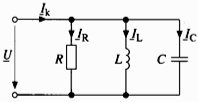
\includegraphics[width=3.5cm]{bilder/Parallelkompensation.png}
        \end{minipage} & 
		Der Kondensator wird parallel dazu geschalten \\ \\
	Zeigerdiagramme Kompensation &
		\begin{minipage}{4.5cm}
        	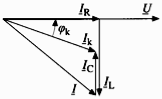
\includegraphics[width=3.5cm]{bilder/Blindstromkompensation.png}
        \end{minipage} &
		\begin{minipage}{4.5cm}
        	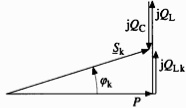
\includegraphics[width=3.5cm]{bilder/Blindleistungskompensation.png}
        \end{minipage} \\ \\
	Neue (kompensierte) Blindleistung &
		$Q_{Lk} = P \cdot \tan{\varphi_k}$ \\
	Blindleistung des Kondensators & 
		\multicolumn{2}{l}{$Q_C = Q_{Lk} - Q_L =  P\cdot (\tan{\varphi_k}-\tan{\varphi}) $} \\
	Kapazität des Kondensators &
		$C = - \frac{Q_C}{\omega U^2}$ \\	
	\end{tabular}
\renewcommand{\arraystretch}{1}
		\begin{multicols}{2}
			\subsubsection{Serieschaltung von $R_S$ \& $X_S$}
				\begin{tabular}{lll}
			%		& $Z = R_S + jX_S$ &\\
			%		& $\varphi = \arctan(\frac{X_S}{R_S})$ & \\
			%		& $U_R = U_0 \cdot \cos\varphi $& \\
			%		& $U_X = U_0 \cdot \sin\varphi $ & \\
			%		& $P = \frac{U_R^2}{R_S} = I^2\cdot R_S$ &\\
			%		& $Q = \frac{U_X^2}{X_S} = I^2\cdot X_S$&
				\end{tabular}
				\begin{align*} 
					Z 		&	= R_S + jX_S 				  \\
					\varphi &	= \arctan(\frac{X_S}{R_S}) 	  \\
					U_R 	&	= U_0 \cdot \cos\varphi 	  \\
					U_X		&	= U_0 \cdot \sin\varphi 	  \\
					P		&	= \frac{{U_R}^2}{R_S} = {I_0}^2\cdot R_S  \\
					Q		&	= \frac{{U_X}^2}{X_S} = {I_0}^2\cdot X_S					
				 \end{align*}
			\columnbreak 
			\subsubsection{Parallelschaltung von $R_P$ \& $X_P$}
				\begin{align*}
					Z 		&	= \frac{1}{\frac{1}{R_P}+j(-\frac{1}{X_P})}	\\
					\varphi &	= \arctan(- \frac{R_P}{X_P})				\\
					I_R 	&	= I_0 \cdot \cos\varphi						\\
					I_X		&	= I_0 \cdot \sin\varphi						\\
					P		&	= \frac{{U_0}^2}{R_P} = {I_R}^2\cdot R_P	    \\
					Q		&	= \frac{{U_0}^2}{X_P} = {I_X}^2\cdot X_P
				\end{align*}
		\end{multicols}

		\subsubsection{Leistungsumsatz bei nichtsinusf\"ormigen periodischen Gr\"ossen}
		\begin{minipage}[c]{7.5cm}
			\parbox{4cm}{Allgemein: Indizes beziehen sich auf Harmonische (Bsp: 0. Har = DC)\\}
			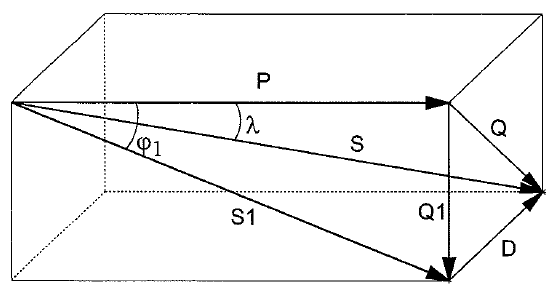
\includegraphics[height=4cm]{bilder/ZeigerdiagrammNichtSinus.png}     
    	\end{minipage}
		\begin{minipage}[c]{10.5cm}   
    		\noindent
    		\renewcommand{\arraystretch}{2.5}
    		\begin{tabular}{p{1.8cm} p{5.6cm}}
        		Unterwelle: 
        			& $X_{U} = \overline{X} = \dfrac{\hat{X}}{\sqrt{2}} a_0 \qquad $  \\
	     		Grundwelle: 
	     			& $X_{G} = \dfrac{\hat{X}}{\sqrt{2}} \sqrt{a_1^2 + b_1^2} \qquad  $   \\
	     		Oberwellen: 
	     			& $X_{O} = \dfrac{\hat{X}}{\sqrt{2}}
	     			\sqrt{\sum\limits_{k=2}^{\infty}a_k^2 +\sum\limits_{k=2}^{\infty}b_k^2}
	     			\qquad $  \\ 
	     		\multicolumn{2}{l}{Effektivwerte: $X_{RMS} = \sqrt{X_G^2 + X_O^2} \qquad X_{TRMS} =
	     			\sqrt{X_U^2 + X_{RMS}^2}$ } \\
				\multicolumn{2}{l}{ges. Blindleistung: 
					$Q = 	\sqrt{Q_G^2 + Q_U^2 + U^2 \sum\limits_{k=2}^{\infty}I_k^2} = \sqrt{U^2 \sum\limits_{k=0}^{\infty}I_k^2}$} \\ 
				\multicolumn{2}{l}{Grundschwinungs-Blindleistung: 
					$Q_1 = \sqrt{{S_1}^2 - P^2}$} \\
				\multicolumn{2}{l}{Wirkleistung: 
					Durch Signale gleicher Frequenz umgesetzt, $P_R = {I_{TRMS}}^2 \cdot R$} \\
				\multicolumn{2}{l}{Verzerrungsblindleistung: 
					$D = U \cdot \sqrt{I_0^2 + \sum\limits_{k=2}^{\infty}I_k^2}$} \\
				\multicolumn{2}{l}{Grundschwinungs-Scheinleistung: 
					$S_1 = U \cdot I_G$} \\
				\multicolumn{2}{l}{ges. Scheinleistung: 
					$S = \sqrt{P^2 + {Q_1}^2 + D^2} = U \cdot I_{TRMS}$} \\
		 	\end{tabular} \\
		 \renewcommand{\arraystretch}{1}
     	\end{minipage}    		\\ \\
     	Die Verzerrungsblindleistung wird von den Oberwellen und ev. von der Unterwelle (je
     	nach Phasenverschiebung) verursacht und ist mit Kondensatoren \textbf{nicht} zu kompensieren -
     	Aktive Filter w\"aren n\"otig.
		\\		
		
	\begin{minipage}[c]{8cm} 
	   \textbf{Beispiel anhand eines Einweggleichrichters:}	  	\\
	   (mit ohmscher Last R) 
	\end{minipage}   
	\begin{minipage}[c]{10cm} 	
	   $ \qquad i(t) = \underbrace{\frac{\hat{I}}{\pi}}_{Unterwelle} + \underbrace{\frac{\hat{I}}{2}
	   \sin(\omega t)}_{Grundwelle} - \underbrace{\frac{2\hat{I}}{\pi} \sum\limits_{k=1}^n \frac{1}{(2k-1)(2k+1)} \cos(2k\omega t)}_{Oberwellen} $
	\end{minipage}   
		
	\begin{minipage}[c]{10cm}  
		\begin{tabular}{| l | l |}
    		\hline 
      		\textbf{Bezeichnung}
      		%& \textbf{N\"aherungsformel}
      		& \textbf{Formel} \\
      		\hline
      		Scheitelwert 
      		%& %& $\hat{I} = 0.7071 \cdot A $
      		& $\hat{I} = \hat{I}_d = \frac{\hat{U}_d}{R} $ \\
      		Unterwelle (Mittelwert)
      		%& $I_U = 0.22508 \cdot A $
      		& $I_U = I_m = \bar{I}_d  = \frac{\hat{I}}{\pi}$ \\
      		Grundwelle
      		%& $I_G = 0.25 \cdot A$ 
      		& $I_G = \frac{\hat{I}}{2 \cdot \sqrt{2}}$ \\
      		Oberwelle
      		%& $I_O = 0.10881 \cdot A$ 
      		& $I_O = \frac{\hat{I}}{\sqrt{2}} \cdot 0.21762$ \\
      		%Effektivwert (RMS)
      		%& $I_{RMS} = 0.27265 \cdot A$
      		%& $I_{RMS} = \sqrt{I_G^2 + I_O^2}$ \\
      		Laststrom
      		%& $I_{TRMS} = 0.35355 \cdot A$
      		& $I_{d} = I_{TRMS} =\frac{\hat{I}_d}{2} = \frac{U_d}{R}$ \\
      		Prim\"arstrom
      		& $I_1 \approx \bar{I}_d \cdot \frac{1.21}{"u}$ \\
      		Leistungen
      		& $Q = D | S_1 = P | Q_1 = 0$ \\
      		%Bauleistung 
      		%& $S_{TR} = \frac{S_{1Tr} + S_{2Tr}}{2}$ \\
      		\hline 
    	\end{tabular}
	\end{minipage}   
	\begin{minipage}[c]{8cm}  
			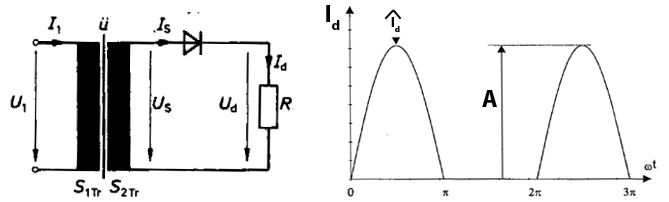
\includegraphics[width=8cm]{bilder/EinwegGR.png}  \\			
	$S_{1Tr} < S_{2Tr}$ da der Trafo keine Gleichstr\"ome übertr\"agt. Somit erscheint der Prim\"arstrom
	als Sekund\"arstrom mit unterdrücktem Gleichstromanteil.\\			
	\end{minipage}

	\begin{minipage}[c]{8cm} 
	   \textbf{Beispiel anhand eines Brückengleichrichters:}	  	\\
	   (mit ohmscher Last R)
	\end{minipage}   
	\begin{minipage}[c]{10cm} 	
	   $ \qquad i(t) = \underbrace{\frac{2 \hat{I}}{\pi}}_{Unterwelle} - \underbrace{\frac{4\hat{I}}{\pi} \sum\limits_{k=1}^n \frac{1}{(2k-1)(2k+1)} \cos(2k\omega t)}_{Oberwellen} $
	\end{minipage}\\
\begin{minipage}[c]{10cm}  
		\begin{tabular}{| l | l |}
    		\hline 
      		\textbf{Bezeichnung}
      		%& \textbf{N\"aherungsformel}
      		& \textbf{Formel} \\
      		\hline
      		Scheitelwert 
      		%& %& $\hat{I} = 0.7071 \cdot A $
      		& $\hat{I} = \hat{I}_d = \frac{\hat{U}_d}{R} $ \\
   %   		Fourien-Reihe
    %  		&$i(t)=A(\frac{2}{\pi}-\frac{4}{\pi}(\frac{\cos(2t)}{1\cdot
 %     		3}+\ldots+\frac{\cos(2nt)}{(2n-1) \cdot (2n+1)}))$\\
      		Unterwelle (Mittelwert)
      		%& $I_U = 0.22508 \cdot A $
      		& $I_U = \bar{I}_d = \frac{2 \hat{I}}{\pi}$ \\
      		Grundwelle
      		%& $I_G = 0.25 \cdot A$ 
      		& $I_G = 0$ \\
      		Oberwelle
      		%& $I_O = 0.10881 \cdot A$ 
      		& $I_O = \frac{\hat{I}}{\sqrt{2}} \cdot 0.43524$ \\
      		%Effektivwert (RMS)
      		%& $I_{RMS} = 0.27265 \cdot A$
      		%& $I_{RMS} = \sqrt{I_G^2 + I_O^2}$ \\ 
      		Laststrom
      		%& $I_{TRMS} = 0.35355 \cdot A$
      		& $I_{d} = I_{TRMS} =  \frac{U_s}{R}= \frac{\hat{U}_d}{\sqrt{2}R}$ \\ 
      		Diodenstrom
      		& $I_{V} = \frac{\hat{U}}{2 R} = \frac{I_{d}}{\sqrt{2}}$ \\
      		Prim\"arstrom
      		& $I_1 \approx \bar{I}_d \cdot \frac{0.966}{"u}$ \\
      	%	Bauleistung 
      	%	& $S_{TR} = \frac{S_{1Tr} + S_{2Tr}}{2}$ \\
      	 	\hline
    	\end{tabular}
	\end{minipage}   
	\begin{minipage}[c]{8cm}  
			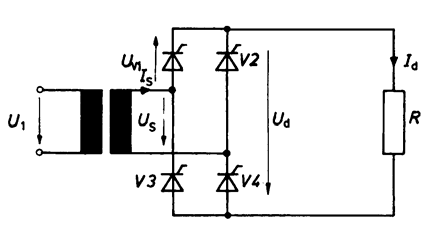
\includegraphics[width=7cm]{bilder/brueckengleichrichter.png}  \\			
	$S_{1Tr} < S_{2Tr}$ da der Trafo keine Gleichstr\"ome übertr\"agt. Somit erscheint der Prim\"arstrom
	als Sekund\"arstrom mit unterdrücktem Gleichstromanteil.			
	\end{minipage}

\section{Transformator}
		
	\subsection{Trafomodelle}
%		\subsubsection{Grundstrucktur des Trafo}
%			\begin{tabular}{p{7cm}p{4.5cm}p{5cm}}
%	        	\textbf{} &
%	        		\begin{minipage}{4.5cm}
%		            	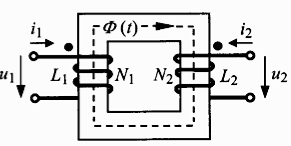
\includegraphics[width=3.5cm]{bilder/GrundstruckturTrafo.png}
%		            \end{minipage} \\
%	        \end{tabular}
		\subsubsection{Der ideale Trafo}
			\begin{tabular}{p{7cm}p{4.5cm}p{5cm}}
				Übersetzungsverh\"altnis &
					$\text{ü} = \frac{|\underline{U}_1|}{|\underline{U}_2|} =
					\frac{|\underline{I}_2|}{|\underline{I}_1|} = \frac{N_1}{N_2}$ &
					\begin{minipage}{4.5cm}
						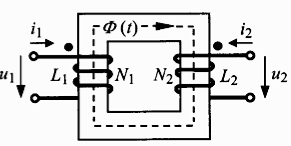
\includegraphics[width=3.5cm]{bilder/GrundstruckturTrafo.png}
					\end{minipage} \\
				Leistungsbilanz &
					$\underline{S}_1 = \underline{S}_2$ &
					oder $\underline{U}_2 \cdot \underline{I}_2^* = \underline{U}_1 \cdot \underline{I}_1^*$ \\
				Scheinwiderstandsübersetztung &
					$\underline{Z}_{aU} = \frac{|\underline{U}_1|^2}{|\underline{U}_2|^2} \cdot \underline{Z}_a = \text{ü}^2 \cdot \underline{Z}_a$ &
					\begin{minipage}{4.5cm}
	            		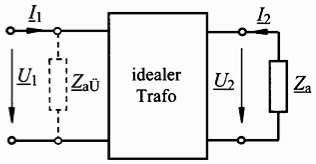
\includegraphics[width=3.5cm]{bilder/IdealerTravoImpedanzwandler.png}
	            	\end{minipage}
			\end{tabular}
		%TODO: 02.02.12 DK, Newpage wieder entfernen wen möglich 
		\newpage
		
		\subsubsection{Verlustloser und Streuungsfreier Trafo}
			\renewcommand{\arraystretch}{1.5}
\textbf{Induktionsgesetz}\\
		\begin{tabular}[c]{p{8.7cm}}
			$u_i= \mp \dot{\Phi} = \mp \frac{d}{dt} \int \vec{B} \cdot
			\vec{dA}\qquad $ \parbox{3cm}{\tiny{$- \Rightarrow B,u_i $
			Rechtsschraube\\ $+ \Rightarrow B,u_i $
			Linksschraube}}
			\\
			
			$u_i= \mp \dot{\Psi}\qquad$ , meist $\; u_i = \mp
			N\cdot\dot{\Phi}$		
		\end{tabular}
		\parbox{8cm}{Durchsetzt das sich \"andernde Magnetfeld einer stromdurchflossenen Spule
					eine zweite Spule, so wird auch in dieser eine Spannung
					(=Gegeninduktionsspannung) induziert.}	

\begin{multicols}{2}
 		\textbf{Gegeninduktion} ($M_{\textcolor{red}{X}\textcolor{green}{Y}}; \textcolor{red}{X}$: Wirkung,
 		$\textcolor{green}{Y}$: Ursache)\\
		\begin{tabular}{ll}
  		Gegeninduktivit\"at
  			& $M_{21} = \frac{\Psi_{m21}}{i_1}$ Meist $= \frac{N_2 \phi_{m21}}{i_1}$\\ 
  			(wenn $\mu$ = const.) & $M = k \cdot \sqrt{L_1 L_2} = M_{21} = M_{12} $  \\
  			Gegeninduktionsspannung
  			& $u_{21} = \dot{\Psi}_{21} = M_{21} \frac{di_1}{dt}$ \\
		\end{tabular}\\

  		\textbf{Transformatorgleichungen}\\
		$\boxed{u_1 = L_1 \dfrac{di_1}{dt} \textcolor{red}{+}\textcolor{green}{-}M_{12}
		\dfrac{di_2}{dt} = L_1 \dfrac{di_1}{dt} \textcolor{red}{-}\textcolor{green}{+}M_{12} \dfrac{di_b}{dt}}$ \\
		$\boxed{u_2 = L_2 \dfrac{di_2}{dt}\textcolor{red}{+}\textcolor{green}{-} M_{21}
		\dfrac{d i_1}{dt} = -L_2 \dfrac{di_b}{dt}
		\textcolor{red}{+}\textcolor{green}{-} M_{21} \dfrac{d i_1}{dt}}$\\
		Im Bildbereich:\\
		$\underline{U}_1 = j\omega\cdot L_1 \cdot \underline{I}_1 + j\omega\cdot M \cdot \underline{I}_2$\\
		$\underline{U}_2 = j\omega\cdot L_2 \cdot \underline{I}_2 + j\omega\cdot M \cdot \underline{I}_1$\\
  			
	  	\textbf{Idealer Trafo}\\ 
	  	$"u = \dfrac{u_1}{u_2} = \dfrac{N_1}{N_2} = \sqrt{\dfrac{L_1}{L_2}}$ $\qquad$ (im Leerlauf:
	  	$\dfrac{1}{"u} = k \sqrt{\dfrac{L_2}{L_1}}$)\\

  		\textbf{Verlustbehafteter Trafo}
  		\begin{list}{$\bullet$}{\setlength{\itemsep}{0cm} \setlength{\parsep}{0cm} \setlength{\topsep}{0cm}} 
          \item Prim\"arstrom im Leerlauf: $L_H$
          	(ideal $L_H \rightarrow \infty)$
          \item Hysterese- \& Wirbelstromverluste: $R_{Fe}$ \newline
          	(ideal: $R_{Fe}\rightarrow \infty$) 
          \item Kupferwiderst\"ande: $R_{Cu1}, R_{Cu2}$
          	(ideal: $R_{Cu}
          \rightarrow 0$)
          \item Streufluss (Kopplung): $L_{\sigma1}, L_{\sigma2}$
          	(ideal: $L_{\sigma} \rightarrow 0$)
        \end{list}

	\columnbreak
  		\begin{flushleft}
  		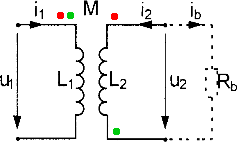
\includegraphics[width=4cm]{bilder/trafo-kopplung.png} \\
  		\small{\textcolor{red}{Gleichsinnig} / \textcolor{green}{Gegensinnig}} \\
  		\vspace{1cm}

	  	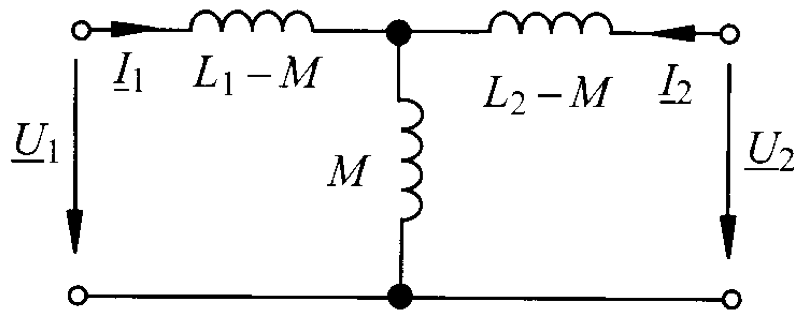
\includegraphics[width=5cm]{bilder/T_Ersatzschaltbild_VST.png}\\
		\end{flushleft}  	
	
\end{multicols}
\renewcommand{\arraystretch}{1} 	
		\subsubsection{Transformatoren-Hauptgleichung (gilt bei Leerlauf)}
			\begin{tabular}{p{7cm}p{4.5cm}p{5cm}}
      			$| \hat{u}_{10} | = \hat{i}_0 \cdot X_{L1}$
      			& 	$\hat{u}_{10} = \hat{i}_0 \cdot \omega \cdot L_1$ \\
      		
				$U_{20} = \frac{2\pi}{\sqrt{2}}N_2 f \hat{B}_1 A$
				&
            	$U_{10} = \frac{2\pi}{\sqrt{2}}N_1 f \hat{B}_1 A$ &
					wobei $\frac{2\pi}{\sqrt{2}} = 4.44$ und $\hat{B} \cdot A = \hat{\Phi}$ 
			\end{tabular}
	\subsection{Der reale (einphasige) Transformator}
		Für dreiphasige Trafos müssen die angegebenen Werte zuerst normiert werden (siehe Kapitel 3).
		\subsubsection{Ersetzen der magnetischen Kopplung}
			\begin{tabular}{p{5.8cm}p{7.3cm}p{4.5cm}}
            	Spannung, Strom &
            		$U_2' = U_2 \cdot \frac{N_1}{N_2}$ \quad 
            		$I_2' = I_2 \cdot \frac{N_2}{N_1}$ \\
            	Nennstrom & 
            		$I_N = S_N / U_N$
            	Widerstand, Streufluss &
            		$R_2' = R_2 \cdot (\frac{N_1}{N_2})^2$ \quad 
            		$X_{\sigma 2}' = X_{\sigma 2} \cdot (\frac{N_1}{N_2})^2$ \\
            	Vollst\"andiges Ersatzschaltbild &
            	\adjustbox{width=6cm}{\begin{circuitikz}[european]
	\draw (0,0) coordinate (In1) {} 
		to[short, *-, i=$\underline{I_1}$] ++(1,0)
		to[R, l=$R_1$] ++(2,0)
		to[L, l=$jX_{\sigma 1}$] ++(2,0)
		to[short, -*] ++(1,0) coordinate (middle1) {}
		to[short] ++(1,0)
		to[L, l=$jX'_{\sigma 2}$] ++(2,0)
		to[R, l=$R'_2$] ++(2,0)
		to[short, -* ,i<=$\underline{I_2}$] ++(1,0) coordinate(Out1);
	\draw (middle1) to[short, -*] ++(0,-1) coordinate (middle2) {};
	\draw (middle2) -- ++(-1,0) 
		to[R, l=$R_{Fe}$] ++(0,-2)
		to[short, -*] ++(1,0) coordinate(middle3)
		to[short, -*] ++(0,-1) coordinate(middle4);
	\draw (middle2) -- ++(1,0)
		to[L, l=$jX_h$] ++(0,-2)
		to[short] (middle3);
	\draw (middle4) to[short, -*] ++(-6,0) coordinate(In2);
	\draw (middle4) to[short, -*] ++(6,0) coordinate(Out2);
	\begin{scope}[
		shorten <=10pt,
		shorten >= 10pt,
		->
	]
		\draw (In1) -- (In2) node[midway, right] {$\underline{U_1}$};
		\draw (Out1) -- (Out2) node[midway, left] {$\underline{U'_2}$};
	\end{scope}
\end{circuitikz}}
            	&
					\begin{minipage}{4.5cm}
                    	\tiny
                    		$R_1, R_2'$: Widerstand Spule\\ \\
                    		$jX_{\sigma 1}, jX_{\sigma 2}'$: Streufluss Spule\\ \\
                    		$R_{Fe}$: Eisenverlust\\ \\
                    		$jX_h$: Hauptfluss Spule\\
                    \end{minipage} \\ \\
				Systemgleichung des realen Trafo &
					$\underline{U}_1 = R_1\cdot\underline{I}_1 + jX_{\sigma 1}\cdot\underline{I}_1 + jX_h\cdot(\underline{I}_1+\underline{I}_2')$ \\
					& $\underline{U}_2' = R_2'\cdot\underline{I}_2' + jX_{\sigma 2}'\cdot\underline{I}_2' + jX_h\cdot(\underline{I}_1+\underline{I}_2')$

            \end{tabular}
            
            	Für mittlere Transformatorenleistungen erbgeben sich etwa folgende Relationen zwischen
            	den einzelnen $R$s und $X$s:
            	$$ R_1 : R_2' : X_{\sigma 1} : X_{\sigma 2}' : X_h : R_{Fe} \approx 1:1:2:2:1000:10000	$$
            	
		\subsubsection{Leerlauf und Magnetisierung}
			\begin{tabular}{p{5cm}p{6cm}p{7cm}}
            	Rechnen &
            		\begin{minipage}{13cm}
                    	Mit Leerlaufdaten $R_{Fe}$ und $X_h$ ausrechnen. $R_1$ und $X_{\sigma1}$ vernachl\"assigen.
                    \end{minipage} \\ \\
            	Induktiver Leerlaufstrom &
            		$\underline{I}_{10} = \underline{I}_{1Fe} + \underline{I}_{1\mu}$ $(\underline{I}_{1\mu} \gg \underline{I}_{1Fe})$ &
            		\begin{minipage}{8cm}
	            		\adjustbox{width=6cm}{\begin{circuitikz}[european]
	\draw (0,0) coordinate (In1) {} 
		to[short, *-, i=$\underline{I}_{10}$] ++(1,0)
		to[R, l=$R_1$] ++(2,0)
		to[L, l=$jX_{\sigma 1}$] ++(2,0)
		to[short, -*] ++(1,0) coordinate (middle1) {}
		to[short, -* ,i<=\mbox{$\underline{I}_2 = 0$}] ++(3,0) coordinate(Out1);
	\draw (middle1) to[short, -*] ++(0,-1) coordinate (middle2) {};
	\draw (middle2) 
		to[short, i_=$\underline{I}_{1Fe}$] ++(-1,0) 
		to[R, l=$R_{Fe}$] ++(0,-2)
		to[short, -*] ++(1,0) coordinate(middle3)
		to[short, -*] ++(0,-1) coordinate(middle4);
	\draw (middle2) 
		to[short, i=$\underline{I}_{1\mu}$] ++(1,0)
		to[L, l=$jX_h$] ++(0,-2)
		to[short] (middle3);
	\draw (middle4) to[short, -*] ++(-6,0) coordinate(In2);
	\draw (middle4) to[short, -*] ++(3,0) coordinate(Out2);
	\begin{scope}[
		shorten <=10pt,
		shorten >= 10pt,
		->
	]
		\draw (In1) -- (In2) node[midway, right] {$\underline{U}_{10}$};
		\draw (Out1) -- (Out2) node[midway, right] {$\underline{U}'_{20}$};
	\end{scope}
\end{circuitikz}}
	            	\end{minipage} \\ \\
				Magnetisierungsstrom &
					$i_\mu = \sqrt{2}I_{\mu1}\cdot \sin(\omega t) + \sqrt{2}I_{\mu3}\cdot \sin(3\omega t) + \sqrt{2}I_{\mu m}\cdot \sin(m\omega t)$ &
					\hspace{3.3cm}$(m=2n+1 \hspace{0.3cm} n\epsilon \mathbb{N}_0)$ \\
					&
					Für den Effektivwert des Stromes: &
					$I_{\mu RMS} = \sqrt{I_{\mu1}^2 + I_{\mu3}^2 +\ldots+ I_{\mu m}} $\\ \\
				Leerlaufverluste &
					$P_0 = P_{0Cu} + P_{0Hy} + P_{0Wi}$ \\
				Hystreseverluste &
					$P_{Hy} \sim f \cdot B^2$ \\
				Wirbelstromverluste &
					$v_W = c_W \cdot f^2 \cdot B^2$ &
					$c_W$ ist materialabh\"angige Konstante \\
				Relativer Leerlaufstrom &
					$i_{0N} = \frac{I_{0N}}{I_{1N}}$ &
					$I_{1N}$ ist eingangsseitiger Nennstrom \\
				Eisenverluststrom &
					$I_{Fe} = \frac{P_{0N}}{U_{1N}} = I_0 \cdot \cos(\varphi_0)$ \\
				Eisenverlustwiderstand &
					$R_{Fe} = \frac{U_{1N}^2}{P_{0N}} = \frac{P_{0N}}{I_{Fe}^2}$ \\
				Hauptreaktanz &
					$X_h = L_h \omega = \frac{U_{1N}}{I_{\mu}} = \frac{U_{1N}^2}{Q_{0N}}
					=
					\frac{Q_{0N}}{I_{\mu}^2}$
					& $Q_{0N} = \sqrt{S_{0N}^2 - P_{0N}^2}$ \\
				Magnetisierungsstrom &
					$I_\mu = I_{0N} \cdot \sin(\varphi_0) = \sqrt{I_0^2 - I_{Fe}^2}$&
					\begin{minipage}{7cm}
                    	\begin{tabular}{p{2.5cm}p{3.5cm}}
	                    	\begin{minipage}{2.5cm}
	                        	\adjustbox{height=1.5cm}{\begin{tikzpicture}
	\begin{scope}[->]
		\draw (0,0) -- +(0,2) node[left] {$\underline{U}_1$};
		\draw (0,0) -- +(2,0) node[below] {$\underline{\Phi}$};
		\draw (0,0.02) -- +(1,0) node[below] {$\underline{I}_\mu$};
		\draw (0,0.02) -- +(1,0.3) node[above] {$\underline{I}_0$};
		\draw (0,0.42) arc (90:16:0.4);
	\end{scope}
	\draw (0.4,0.5) node {$\varphi_0$};	
\end{tikzpicture}%}
	                        \end{minipage} &
							\begin{minipage}{3.5cm}
	                       		oder $\hat{I}_{\mu} = \frac{\hat{H}_{Fe} \cdot l_{Fe}}{N_1}$
	                        \end{minipage}
						\end{tabular}
	            	\end{minipage} \\
				Leistungsfaktor im Leerlauf &
					$\cos(\varphi_0) = \frac{P_{0N}}{I_{0N} \cdot U_{1N}}$ \\
            \end{tabular}
		\subsubsection{Kurzschluss}
			\begin{tabular}{p{5cm}p{6cm}p{7cm}}
				\multicolumn{2}{p{11cm}} {
					Mit Kurzschlussdaten $R_1$ und $X_{\sigma1}$ ausrechnen. $R_{Fe}$ und $X_h$ vernachl\"assigen.
				}
				& \multirow{3}{*}{
	            	\adjustbox{width=6.5cm}{\begin{circuitikz}[european]
	\draw (0,0) node (in) {} to[short, *-, i=$\underline{I_1}$] ++(1,0)
		to[R, l=$R_1$] ++ (2,0)
		to[L, l=$jX_{\sigma 1}$] ++(2,0)
		to[L, l=$jX^`_{\sigma 2}$] ++(2,0)
		to[R, l=$R^`_2 $] ++(2,0)
		-- ++(0,-2) to[short, -*] (0,-2) node (out) {};
	\draw[shorten >= 5pt, shorten <= 5pt, ->] (in) -- (out)
		node[midway, right] {$\underline{U_1}$};	
\end{circuitikz}}
	              }
	            \\
				Kurzschlussimpedanz&
					$\underline{Z}_k = R_k + jX_k$ \\
					& $Z_k = \frac{U_k}{I_k}$ \\
					& $R_k = R_1 + R_2' = \cos{\varphi_k} \cdot Z_k  = \frac{P_k}{I_k^2}$  \\
					& $X_k = X_{\sigma1} + X_{\sigma2}' = \sin{\varphi_k} \cdot Z_k = \frac{Q_k}{I_k^2}$ \\
				Leistungsfaktor im Kurzschluss&
					$\cos(\varphi_k) = \frac{P_k}{U_k \cdot I_k} = \frac{P_k}{S_k}$ \\
             \end{tabular}

		\subsubsection{Spannungs\"anderung bei Belastung}
			\begin{tabular}{p{10cm}p{6cm}}
            		\begin{minipage}{10cm}
	            		$\underline{U}_1 =
	            		\underline{U}_R+\underline{U}_X+\underline{U}_2'$ \qquad
	            		$\underline{U}_2'=\underline{U}_2 \cdot "u$\\ \\
	            		$\underline{U}_R=R_k \cdot \underline{I}_1$ \qquad
	            		$\underline{U}_X=jX_k \cdot \underline{I}_1$\qquad
	            		$\underline{I}_2' = \underline{I}_1$\\
	            		\end{minipage} &
            		\begin{minipage}{6cm}
	            		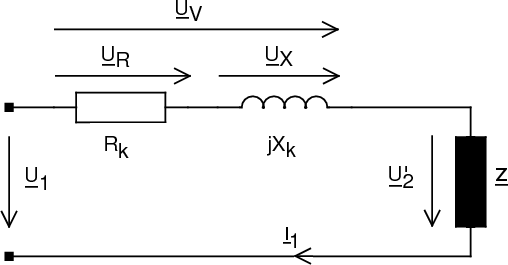
\includegraphics[width=5cm]{bilder/ErsatzschaltbildTrafoLast.png}
	            	\end{minipage}\\			
            \end{tabular}\\ \\

			\begin{tabular}{p{8cm}|p{10cm}}
	 			\textbf{Zeigerdiagramme} & \textbf{Kappsches Dreieck}\\
				\begin{minipage}{8cm}
	            	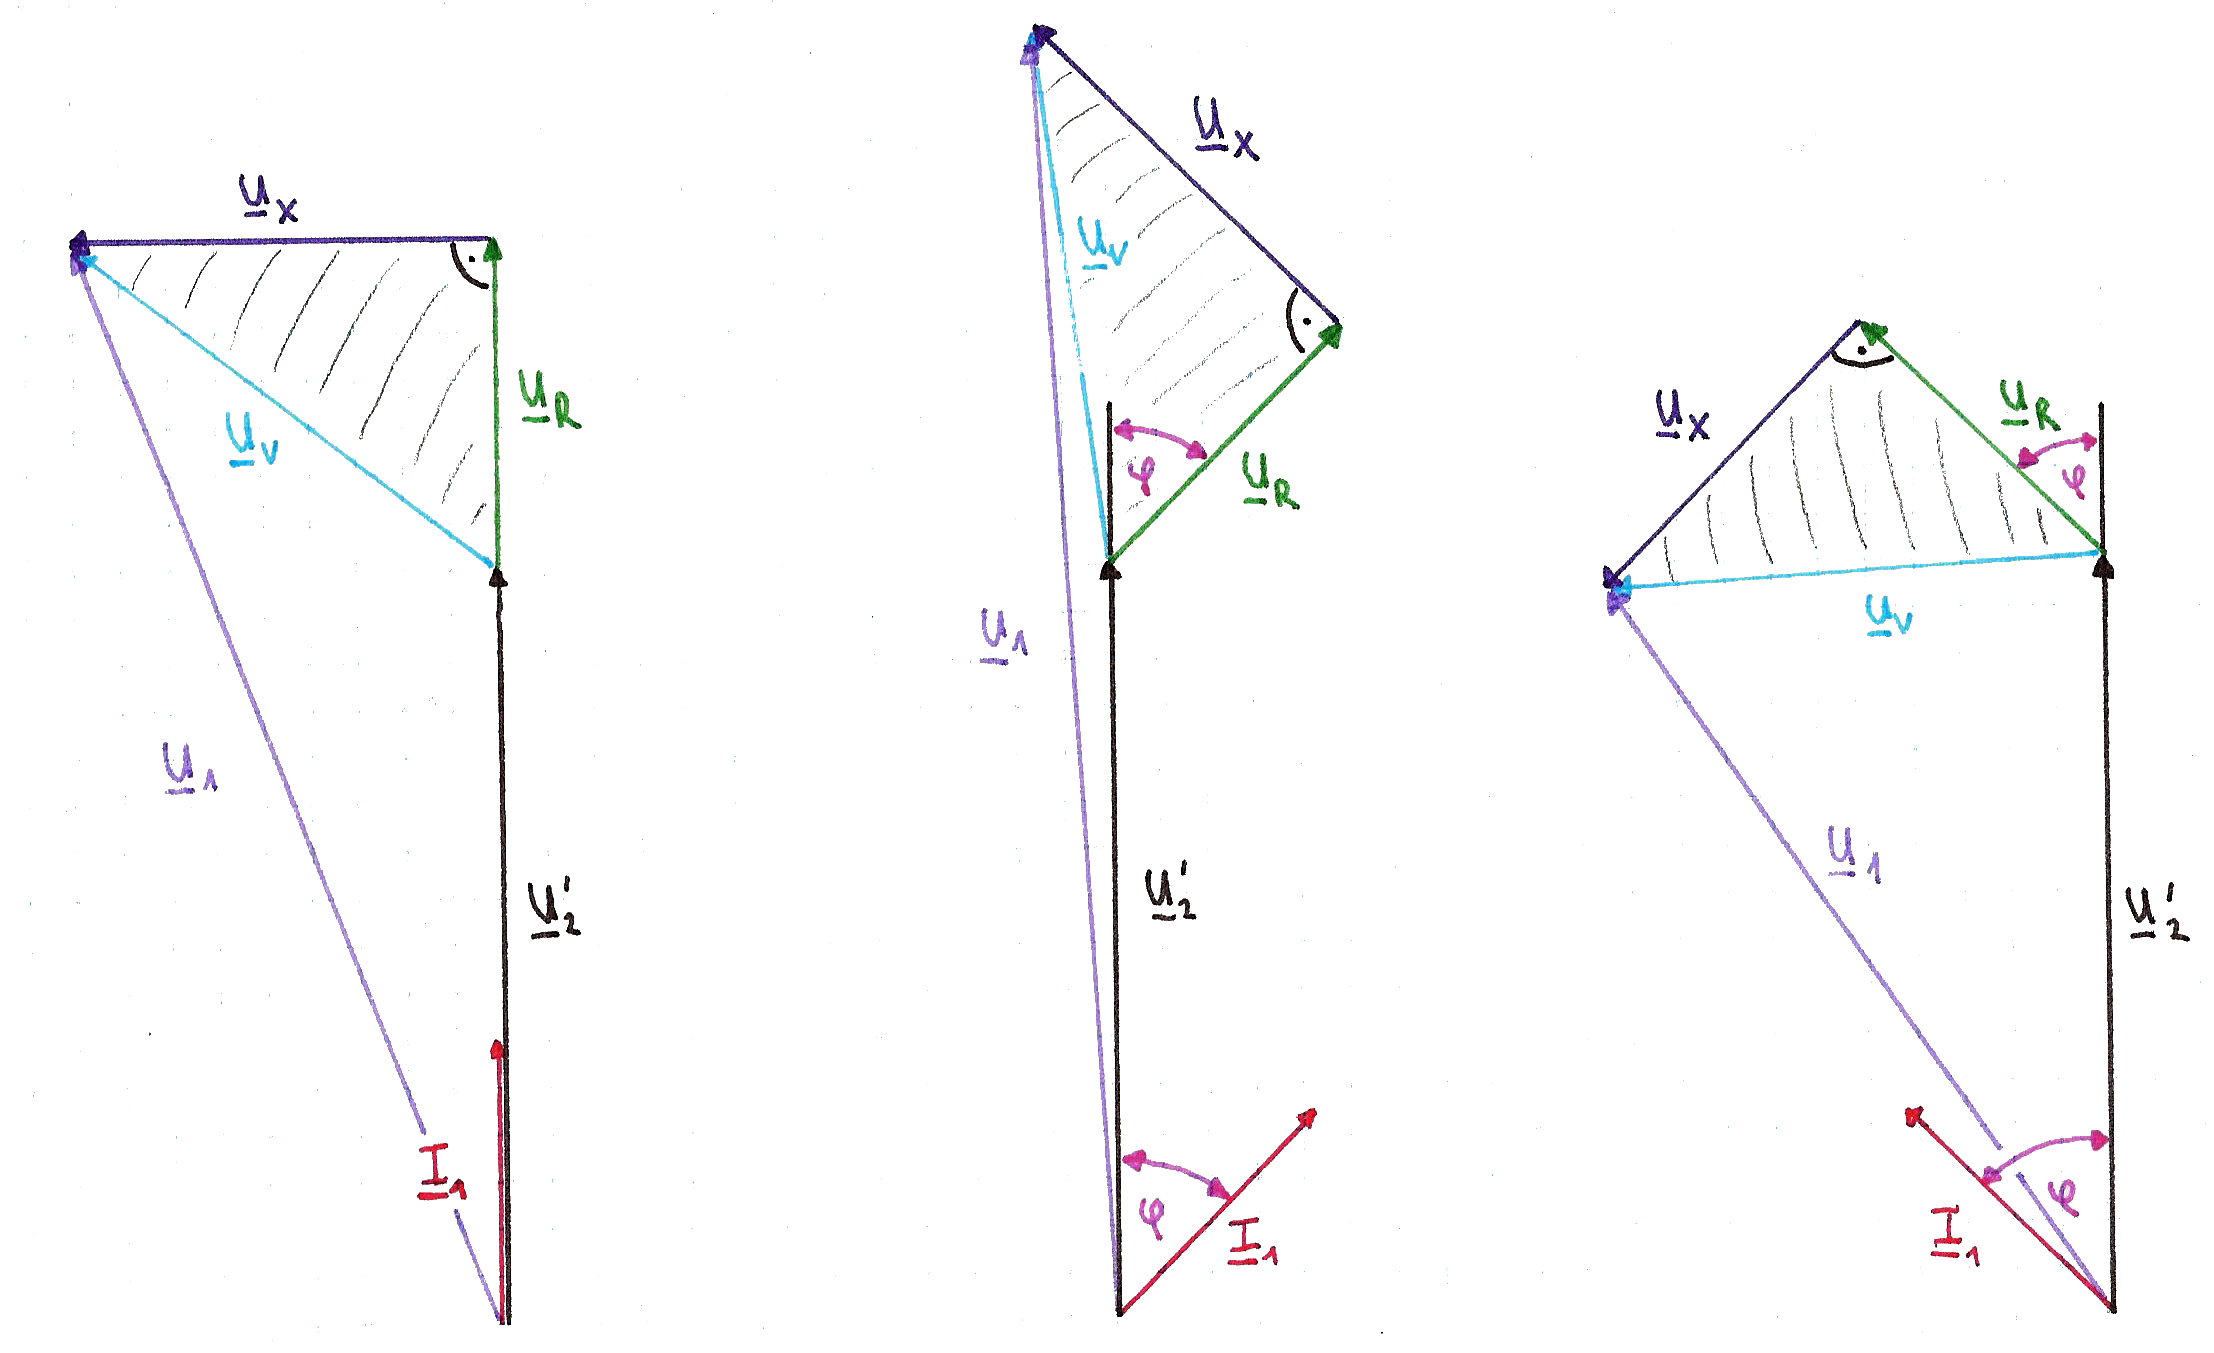
\includegraphics[width=8cm]{bilder/KappschesDreieck_1.png}
	            \end{minipage}  & \hspace{0.2cm}
				\begin{minipage}{10cm} 
		        	\begin{minipage}{2.5cm}
						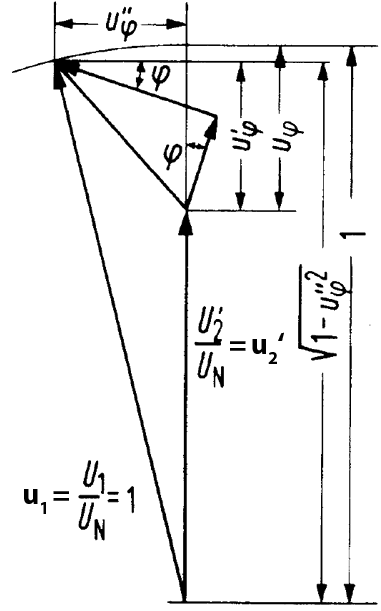
\includegraphics[width=3cm]{bilder/KappschesDreieck.png}
		            \end{minipage}
					\begin{minipage}{7.5cm}
		      			$$u_{\varphi} = u_{\varphi'} + 1 - \sqrt{1 - u_{\varphi''}^2}$$
		      			$$ u_\varphi \approx u_{\varphi'}\quad (\text{für }u_k
		      			=\frac{U_k}{U_{N}} \cdot 100\% < 4 \%)$$
		      			$$u_{\varphi'} = u_r \cdot \cos \varphi + u_x
		      			\cdot \sin \varphi$$ $$u_{\varphi''} = u_x \cdot \cos \varphi - u_r \cdot \sin \varphi$$
		      			$$ u_r = \frac{R_k I}{U_N} \qquad u_x = \frac{X_k I}{U_N} $$
		      			$$ U_2 = \frac{U_N}{"u} - \Delta U_2 = \frac{U_1}{"u} - \frac{1}{"u}
		      			U_N u_\varphi $$\\
		      		\end{minipage}         
                \end{minipage}\\
				\begin{minipage}{8cm}
 					\begin{tabular}[c]{p{2.66cm}p{2.66cm}p{2.66cm}}
                     	$\quad \varphi = 0$ & $\quad\varphi > 0$ & $\quad\varphi
                     	< 0$\\ rein ohmsche & induktive & kapazitive\\
                     	Last & Last & Last\\
                     	&&\\
                     	&&\\
                     	&&\\
                     	&&\\
                     \end{tabular}               
                \end{minipage}& \hspace{0.2cm}
				\begin{minipage}{10cm}
		      		Beim kappschen Dreieck wird mit ``genormten'' Gr\"ossen (klein $u$) gerechnet: 
		      		$u = \frac{U_{Strang}}{U_{N, Strang}} = \frac{U_X}{U_1} \qquad
		      		\boldsymbol{U_N = U_1} $\\ \\ Das Kappsche Dreieck dreht sich um die
		      		Spitze der Prim\"arspannung. Bei konstantem Strom und variablem $cos(\varphi)$ beschreibt ${u}_2'$
		      		einen
		      		Kreis um die Prim\"arspannung.\\ Bei \textbf{kapazitiver Last steigt}
		      		die Sekund\"arspannung über den Leerlaufwert an. \\                  
                \end{minipage}     
            \end{tabular}

		
		\subsubsection{Wirkungsgrad des Trafos}
			\begin{tabular}{p{5cm}p{7cm}p{7cm}}
            	Wirkungsgrad &
            		$\eta = 1-\dfrac{P_{V0} + P_{VK} \cdot
            		(\frac{P_B}{P_N})^2}{P_B} $ &
            	\begin{minipage}{7cm}
                	$P_B$ = Betriebsnennleistung\\
                	$P_{N}$ = Nennleistung\\
                	$P_{V0}$ = Leerlaufverlustleistung\\
                	$P_{VK}$ = Kurzschlussverlustleistung                	
                \end{minipage}\\ \\
            	 &
            		$\eta = 1 - \dfrac{a + (\frac{P_B}{P_N})^2}{P_B} P_{VK}$ &
            	\begin{minipage}{7cm}
 					$a = \dfrac{P_{V0}}{P_{VK}}$                	
                \end{minipage}\\ \\            		
            	 &
            		$\eta = 1 - \frac{P_{V0}+P_{VK}}{P_B} $ 
            		& (bei Wirkleistungsvollast) \\ \\
            	Maximaler Wirkungsgrad
            	& $S_{\eta-max} = \sqrt{a} \cdot S_N$ $P_{\eta-max} = \sqrt{a}
            	\cdot P_N$
            	& (Kupferverluste = Eisenverluste)
            \end{tabular}	

\newpage
	\subsection{Transformatoren Kühlmittel}
		\begin{center}
	    	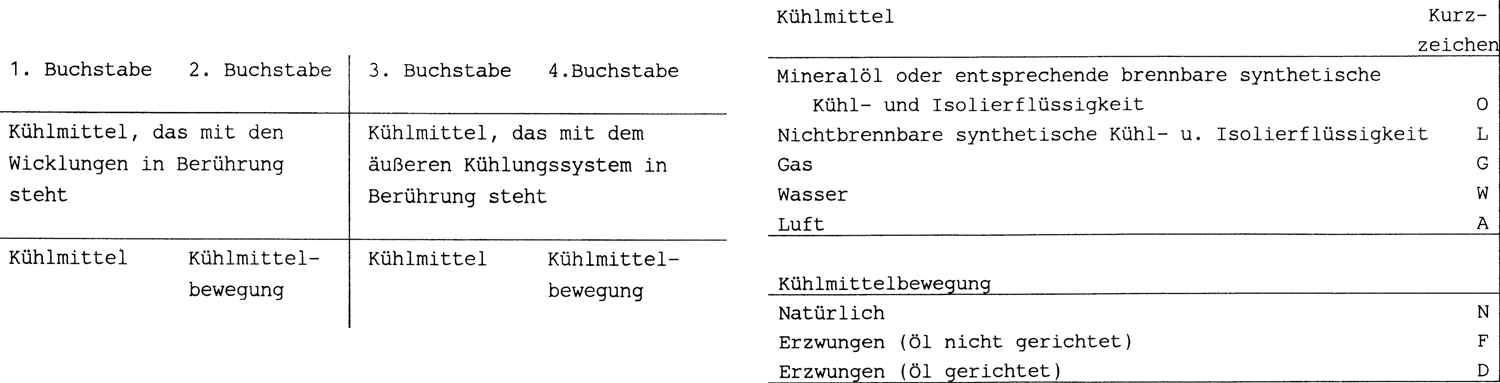
\includegraphics[width=19cm]{bilder/Kuehlmittel.png}
	    \end{center} 

	\subsection{Drehstrom-Leistungstransformatoren} 
	Angegebene Leistung bezieht sich immer auf alle drei Wicklungen. $\Rightarrow P_{Wicklung} =
	\frac{P_N}{3}$ \\
	Angegebene Spannungen und Str\"ome gelten immer für Aussenleiter. Somit muss immer entweder - je
 nachdem ob Dreieck- oder Sternschaltung vorliegt -	Strom oder Spannung mit Faktor
 $\frac{1}{\sqrt{3}}$ multipliziert werden.
 	\subsubsection{Bauformen}
	 $$\text{Kennzeichnung} = [a][b][c][d] = \begin{cases}
                  [a] = \text{Oberspannungswicklung, Grossbuchstabe (Y,D,III,Z)
                  }\\
                  [b] = \text{Unterspannungswicklung, Kleinbuchstabe (y,d,iii,z) } \\
                  [c] \cdot 30^\circ = \text{Phasenverschiebung zwischen Unter- und Oberspannung }
                  \\ [d] = 0 \text{, falls Neutralleiter herausgeführt (optional)}
                  \end{cases}$$
		\begin{center}
	    	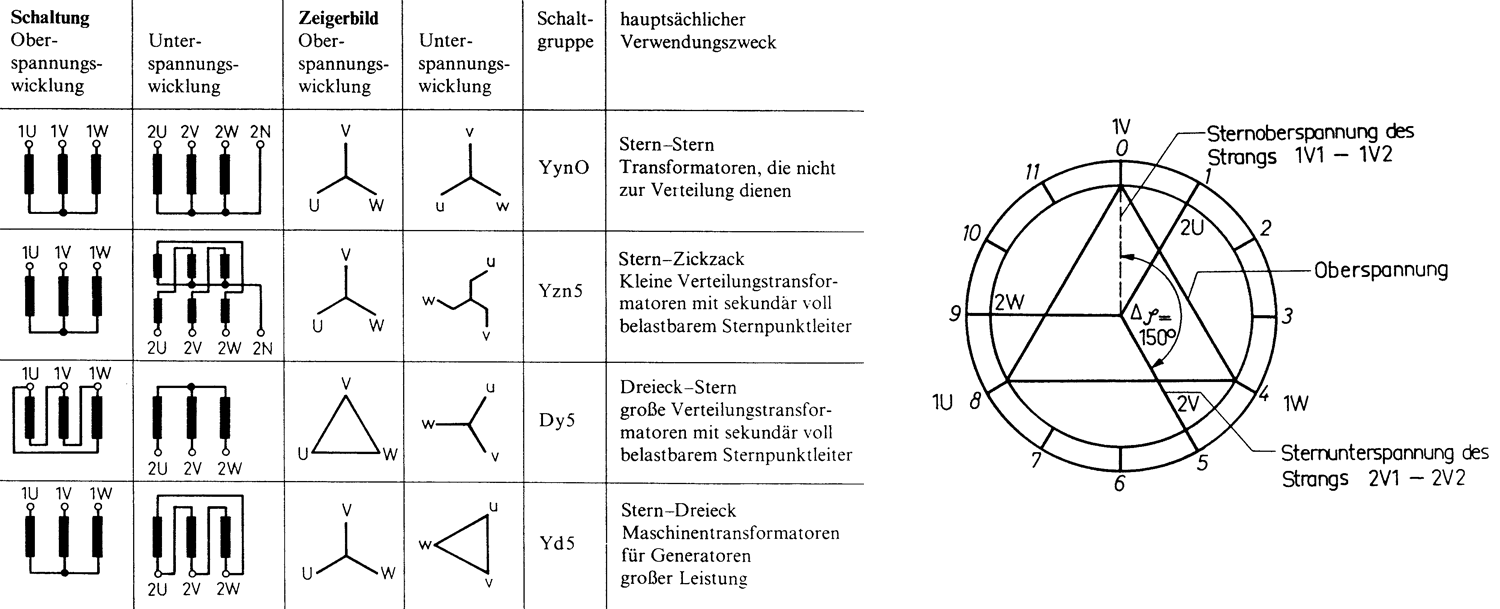
\includegraphics[height=6cm]{bilder/Drehstromtrafo.png}
	    \end{center} 

\section{Dreiphasenwechselstrom (Drehstrom)}
	%\subsection{Entstehung des Drehstrom-Systems}
		\begin{tabular}{p{8.5cm}p{9cm}}
        	\begin{minipage}{8cm}
            	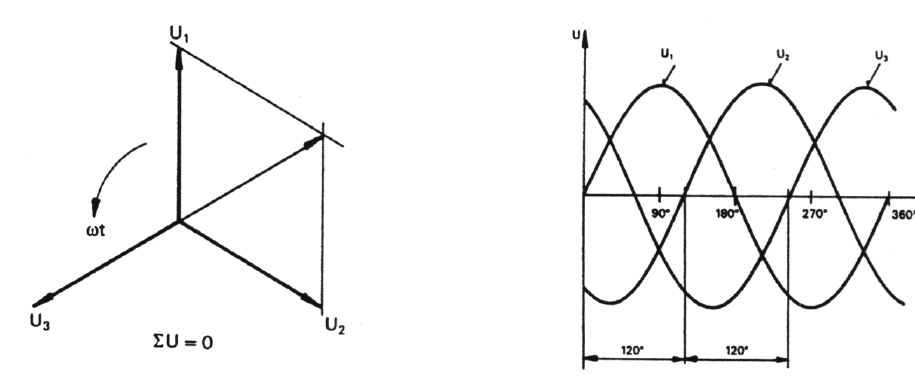
\includegraphics[width=7.5cm]{../WS_DST/bilder/Drehstrom.png}
            \end{minipage} &    
			\begin{minipage}{10cm}
            	Zeiger drehen mit $\omega t$ im Gegenuhrzeigersinn ($\omega > 0$). \\
            	$\underline{U}_2$ ist gegenüber $\underline{U}_1$ 
				$120^{\circ}$ nacheilend, $\underline{U}_3$ gegenüber $\underline{U}_1$ $240^{\circ}$.  \\ \\
				Somit gilt (bei symmetrischer Belastung): \\
				$\underline{U}_2 = \underline{U}_1 \cdot e^{j (-120^{\circ})}; \underline{U}_3
				= \underline{U}_1 \cdot e^{j (-240^{\circ})} = \underline{U}_1 \cdot e^{j
				(120^{\circ})}$
            \end{minipage}
        \end{tabular}
		
% 		\subsubsection{Verketten der Spannungen oder Str\"ome}
% 			\begin{tabular}{p{5cm}p{6cm}p{7cm}}
%             	\textbf{Maschensatz} &
%             		\fbox{$\underline{U}_1 + \underline{U}_2 + \underline{U}_3 = 0$} \\
%             	\textbf{Knotenpunktsatz} &
%             		\fbox{$\underline{I}_1 + \underline{I}_2 + \underline{I}_3 = 0$} \\
%             \end{tabular}

		\subsubsection{Stern- (Y) / Dreieckschaltung ($\Delta$)}
            	\renewcommand{\arraystretch}{1.5}
			\begin{tabular}{| p{4.5cm} | l | l |}
				\hline
	 				& Sternschaltung (Y)		& Dreieckschaltung ($\Delta$)\\
	 			\hline
	 			\vspace{0.2cm}
	 				%\textbf{Zeigerdiagramm} & & \\ 
	 				&
	 					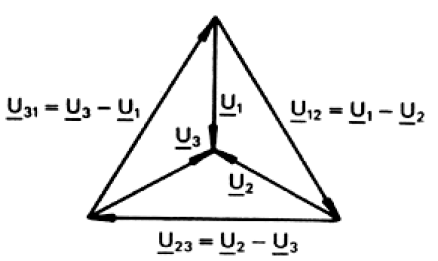
\includegraphics[width=5cm]{../WS_DST/bilder/Sternspannung.png} &
	 					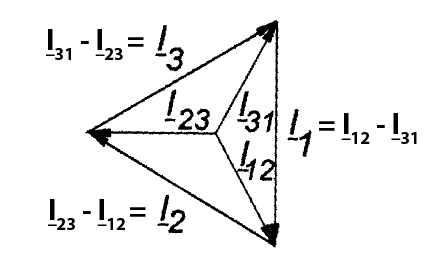
\includegraphics[width=5cm]{../WS_DST/bilder/Dreieckstrom.png} \\
	 				
		 			Verkettete Spannung &
		 				$U = U_{Str} \cdot \sqrt{3}$ \hspace{0.2cm} $\underline{U} = \underline{U}_{Str} \cdot \sqrt{3} \cdot e^{j 30^\circ}$ &
		 				$U = U_{Str}$ \hspace{0.2cm} $\underline{U} = \underline{U}_{Str}$ \\
		 			Aussenleiterstr\"ome &
		 				$I = I_{Str}$ \hspace{0.2cm} $\underline{I} = \underline{I}_{Str}$ &
		 				$I = I_{Str} \cdot \sqrt{3} $ \hspace{0.2cm} $\underline{I} =
		 				\underline{I}_{Str} \cdot \sqrt{3} \cdot e^{-j 30^\circ} $ \\ Gesamt-Scheinleistung &
		 				$S = 3 \cdot S_{Str} =\sqrt{3} \cdot U \cdot I $ \hspace{0.2cm} in $[VA]$
		 				& $S = 3 \cdot S_{Str} = \sqrt{3} \cdot U \cdot I$ \hspace{0.2cm} in $[VA]$ \\ Scheinleistung pro Strang &
		 				\multicolumn{2}{l|}{\hspace{3cm} $S_{Str} = U_{Str} \cdot I_{Str}$ \hspace{0.2cm} in $[VA]$} \\
		 			Wirkleistung &
		 				\multicolumn{2}{l|}{\hspace{3cm} $P = S \cdot \cos\varphi = \sqrt{3} \cdot U \cdot I \cdot \cos\varphi$ \hspace{0.2cm} in $[W]$} \\
		 			Blindleistung &
		 				\multicolumn{2}{l|}{\hspace{3cm} $Q = S \cdot \sin\varphi = \sqrt{3} \cdot U \cdot I \cdot \sin\varphi$ \hspace{0.2cm} in $[var]$} \\
% 		 			Wirkarbeit &
% 		 				\multicolumn{2}{l|}{\hspace{3cm} $W = P \cdot t = \sqrt{3} \cdot U \cdot I \cdot cos\varphi \cdot t$ \hspace{0.2cm} in $[Ws, kWh]$} \\
% 		 				&\multicolumn{2}{c|}{}\\
% 		 			Blindarbeit &
% 		 				\multicolumn{2}{l|}{\hspace{3cm} $W_b = Q \cdot t = \sqrt{3} \cdot U \cdot I \cdot sin\varphi \cdot t$ \hspace{0.2cm} in $[varh, kvarh]$} \\
	 			\hline
			\end{tabular}
        \renewcommand{\arraystretch}{1}
		
		%\subsubsection{Bestimmung des Y-Punktes mittels Leitwert-Operatoren im Vierleiter-Drehstromnetz}
        \subsubsection{Ausfall des Neutralleiters: Bestimmung des Y-Punktes mittels Leitwert-Operatoren}
            \begin{tabular}{p{5cm}p{13cm}}
            	\begin{minipage}{8cm}
                	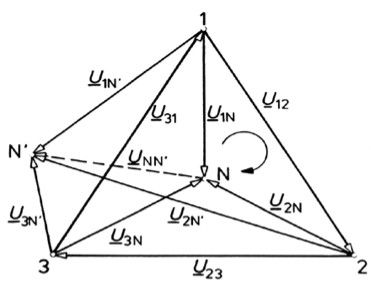
\includegraphics[width=5cm]{../WS_DST/bilder/ZeigerdarstellungVerschobenerSternpunkt.png}
                \end{minipage} &
				\begin{minipage}{13cm}
                	$\underline{U}_{12} = \underline{U}_{1N'} - \underline{U}_{2N'}$ \hspace{0.3cm}
                	$\underline{U}_{1N'} = \underline{U}_{1N} + \underline{U}_{NN'}$ \hspace{0.3cm}
                	$\underline{I}_1 = \underline{Y}_1 \cdot \underline{U}_{1N'} = \underline{Y}_1 \cdot (\underline{U}_{1N} + \underline{U}_{NN'})$ \\
                	$\underline{U}_{23} = \underline{U}_{2N'} - \underline{U}_{3N'}$ \hspace{0.3cm}
                	$\underline{U}_{2N'} = \underline{U}_{2N} + \underline{U}_{NN'}$ \hspace{0.3cm}
                	$\underline{I}_2 = \underline{Y}_2 \cdot \underline{U}_{2N'} = \underline{Y}_2
                	\cdot (\underline{U}_{2N} + \underline{U}_{NN'})$ \\ $\underline{U}_{31} = \underline{U}_{3N'} - \underline{U}_{1N'}$ \hspace{0.3cm}
                	$\underline{U}_{3N'} = \underline{U}_{3N} + \underline{U}_{NN'}$ \hspace{0.3cm}
                	$\underline{I}_3 = \underline{Y}_3 \cdot \underline{U}_{3N'} = \underline{Y}_3
                	\cdot (\underline{U}_{3N} + \underline{U}_{NN'})$ \\ \\ 
                	$$\underline{U}_{NN'} = \boldsymbol{-} \frac{(\underline{Y}_1 \cdot
                	\underline{U}_{1N} + \underline{Y}_2 \cdot \underline{U}_{2N} + \underline{Y}_3 \cdot
                	\underline{U}_{3N})}{\underline{Y}_1 + \underline{Y}_2 +
                	\underline{Y}_3}$$
                \end{minipage}
			\end{tabular}

%		\subsubsection{Anwendung der Y- und $\Delta$- Schaltung}
	
	\subsection{Stern-Dreieck-Umwandlung}% \formelbuch{18}}
	%\begin{figure}
	  \begin{minipage}[lt]{7.5 cm}
	    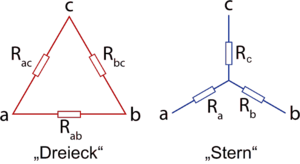
\includegraphics[width=6cm]{bilder/stern-dreieck.png} 
	  \end{minipage}
	  \begin{minipage}[rt]{9.35 cm} %BASTEL!!
      \renewcommand{\arraystretch}{2}
	  \begin{tabular}{ll}
	Umwandlung $\triangle \rightarrow Y$: 
		&$Z_{c} = \dfrac{Z_{ac} Z_{bc}}{Z_{ab}+Z_{bc}+Z_{ac}}$\\
	Umwandlung $Y \rightarrow \triangle$: 
		&$Y_{ac}=\dfrac{Y_{a} Y_{c}}{Y_{a}+Y_{b}+Y_{c}}$\\
	Bei gleichen Widerst\"anden:
	&$R_Y = \frac{R_\triangle}{3}$ \\
	Bei gleichen Kapazit\"aten:
	&$C_Y = C_\triangle \cdot 3 $ \\
	Bei gleichen Induktivit\"aten:
	&$L_Y = \frac{L_\triangle}{3}$
	  \end{tabular}
      \renewcommand{\arraystretch}{1}
	  \end{minipage}
	%\end{figure}
	
	\subsection{Defektleistung von symmetrischen Drehstromverbrauchern}
		\begin{tabular}{| p{7.5cm} | l | l |}
			\hline
 				& Normalleistung		& Defektleistung\\
 			\hline
	 			\textbf{Y-Schaltung bei Leiter- oder Strangausfall} ohne Neutralleiter &
	 				$P_{Norm} = 3 \cdot \frac{U^2_{Str}}{R} = \frac{U^2}{R}$ &
	 				$P_{Def} = \frac{1}{2} \frac{U^2}{R}$ \tiny{nur 50\% von $P_{Norm}$} \\
	 			&&\\
	 			\textbf{Y-Schaltung bei Leiter- oder Strangausfall} mit Neutralleiter &
	 				$P_{Norm} = 3 \cdot \frac{U^2_{Str}}{R} = \frac{U^2}{R}$ &
	 				$P_{Def} = 2 \cdot \frac{U^2_{Str}}{R} = \frac{2}{3} \frac{U^2}{R}$ \tiny{nur 66\% von
	 				$P_{Norm}$} \\ &&\\
	 			\textbf{$\Delta$-Schaltung bei Leiterausfall} &
	 				$P_{Norm} = 3 \cdot \frac{U^2}{R}$ &
	 				$P_{Def} = \frac{U^2}{R} + \frac{U^2}{2R} = \frac{3U^2}{2R}$ \tiny{nur 50\% von $P_{Norm}$} \\
	 			&&\\
	 			\textbf{$\Delta$-Schaltung bei Strangausfall} &
	 				$P_{Norm} = 3 \cdot \frac{U^2}{R}$ &
	 				$P_{Def} = 2 \cdot \frac{U^2}{R}$ \tiny{nur 66\% von $P_{Norm}$} \\
	 		\hline
		 \end{tabular} 

\input{idiotenseite/trigo/trigoInclude}
\input{idiotenseite/elektrotechnik/subsections/ohmscheLeistung}
\input{idiotenseite/elektrotechnik/subsections/signalformen}
%\input{idiotenseite/diverses/subsections/idiotenformel}
\input{idiotenseite/diverses/subsections/sivorsaetze}
%\input{idiotenseite/diverses/subsections/unbestimmteIntegrale}
% 	\subsection{Messen der Drehstromleistung}
% 	\subsection{Kompensation im Drehstromnetz}
%%%%%%%%%%%%%%%%%%%%%%%%%%%%%%%%%%%%%%%%%%%%%%%%%%%%%%%%%%%%%%%%%%%%%%%%%%%%%%%%%%%%%%%%%%%%%%%%	
% \section{Komplexe Zahlen mit Taschenrecher - Texas Instruments}
% 	\begin{tabular}{p{4cm}p{10cm}}
% 	$\ldots \triangleright Rect $ 		& Umwandlung in Kartesische Darstellung \\
% 	$\ldots \triangleright Polar $ 		& Umwandlung in Polare Darstellung \\
% 	$conj(\ldots)$ 						& Konjugiert Komplex $\overline{z}$\\
% 	$abs(\ldots) $						& Betrag $|z|$\\
% 	$angle(\ldots) $					& Winkel $arg(z)$\\
% 	$imag(\ldots) $	s					& Imagin\"arteil $Im(z)$ \\
% 	$real(\ldots) $						& Realteil $Re(z)$ \\
% 	\end{tabular}

%%%%%%%%%%%%%%%%%%%%%%%%%%%%%%%%%%%%%%%%%%%%%%%%%%%%%%%%%%%%%%%%%%%%%%%%%%%%%%%%%%%%%%%%%%%%%%%%
%%%%%%%%%%%%%%%%%%%%%%%%%%%%%%%%%%%%%%%%%%%%%%%%%%%%%%%%%%%%%%%%%%%%%%%%%%%%%%%%%%%%%%%%%%%%%%%%


\end{document}